\section{Design and Implementation: Communication}
\label{sec:communication}
The implementation of the communication system required the selection of a suitable communication technique prior to implementation.
Because each Truck needs to be able to communicate with every other Truck, the resulting communication scenario is a N-to-N scenario.
This had a major impact on the elicitation of a suitable communication technique as the technique needs to support such a case.
Since the whole project is mostly written in C++ and executed on Windows machines, the usage of a TCP/IP connection by using the winsock2.h library
was an obvious choice.

\par

The communication scenario and the working principle of the winsock2.h library had a major influence on the resulting network topology. Because of
the N-to-N scenario and the lacking possibility of realizing a “discovery procedure” (initialization phase of nodes of a wireless network) with the
TCP/IP protocol, a client server architecture of the network was chosen.
\begin{figure}[ht]
    \centering
    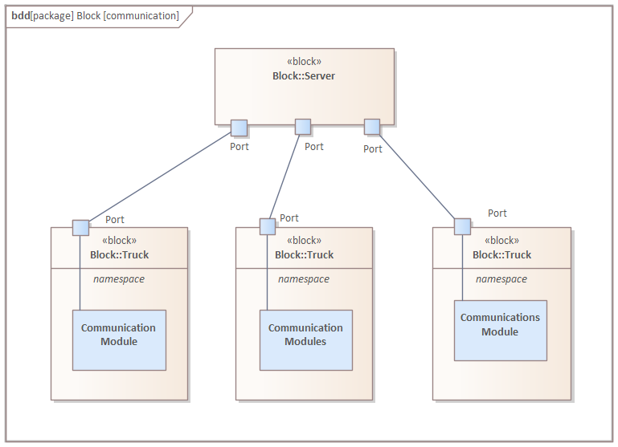
\includegraphics[width=0.5\textwidth]{images/comms_architecture.png}
    \caption{Architecture of the communication system}
    \label{img:comms_arch}
\end{figure}

\subsection{Implementation of the server}
Because of the working principle of the server of being independent to the rest of the simulation, it
was developed as an own application. After some experiments with the winsock2.h library, the needed key
features of the server were found out:
\begin{itemize}
    \item Accepting new connections.
    \item Receiving messages from the clients.
    \item Forwarding messages to their destination.
    \item Supplying all connected clients with an overview of all reachable clients.
\end{itemize}
With these needed features in mind, a simple activity diagram of the servers’ working procedure was
developed.
\begin{figure}[ht]
    \centering
    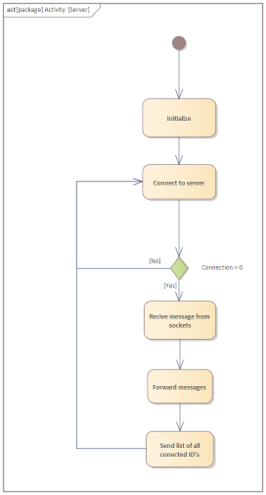
\includegraphics[width=0.25\textwidth]{images/comms_server_act.png}
    \caption{Working principle of the server}
    \label{img:comms_server_principle}
\end{figure}
The idea was to use a sequential way of processing the packets. After the initialization of the server
and especially the socket that all clients try to connect to, it polls the socket for new incoming
connections. If there is a connection available, it is accepted, and the resulting socket is stored into
a vector. For this vector, the struct “SocketClientID” was created. It contains two fields:
\begin{itemize}
    \item clientSocket [SOCKET]: used to store the socket of the client.
    \item ID [int]: used to associate the trucks’ ID of the client to the socket.
\end{itemize}
When the connection is accepted, the value of the field “ID” is left at the default of 0 as there is at
this point no information which ID the truck has. This information gets filled in with the first
received packet as the packet contains the ID of the sender.

\par
\medskip
After polling for new connections, the server checks if there is at least one active connection.
If not, it continues to poll for new connections. Otherwise, the server polls all sockets of the
elements of the vector for incoming packets. When there is a packet received, the field “ID” of the
vector’s element is checked, if there is already an associated ID. If not, the sender ID is extracted
from the message and written to the field. In any case, the message is then stored into a buffer. After
all messages are received and stored, the server proceeds with the forwarding of the messages. This
incorporates the extraction of the destination ID from the message to search for the receivers’ socket
in the vector that contains the sockets of all connected clients together with their ID. If the matching
socket was found, the message gets forwarded. As a last step, a message that contains all the IDs of all
connected clients is created and sent to all clients.

\par
\medskip
These steps were implemented as separate functions called “initialize”, “checkAndAcceptConnection”,
“getMessagesFromAllSockets”, “forwardPackets” and “sendClientIDVector”. In the main loop, they are
called in this sequence to ensure the proper operation of the server. The modularity allowed a
structured development and made it simple to expand the functionalities. This came in hand when the
feature of sending the information about all connected clients was added after the first version of the
server was already developed.

\subsection{Implementation of the client}
The matching counterpart to the server, the communication module of the truck, was designed work in a
similar way. Since the responsibilities of client and server were separated before the implementation,
it was clear, that the communication module needs to support the following features:
\begin{itemize}
    \item Initializing the communication and connecting to the server.
    \item Sending a buffer of messages that should be transmitted.
    \item Receiving messages and storing them into a buffer.
    \item Being able to add messages to and to get messages from the buffers.
    \item Supplying a list of all reachable clients to the controller.
\end{itemize}
A simple activity diagram to visualize the communication modules’ working
principle was created:
\begin{figure}[ht]
    \centering
    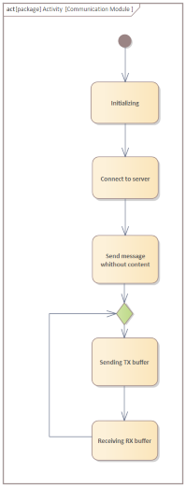
\includegraphics[width=0.25\textwidth]{images/comms_client_act.png}
    \caption{Working principle of the client}
    \label{img:comms_client_principle}
\end{figure}
The whole process was also designed to be sequential. After the initialization of the clients’ socket, a
connection to the server is established. To allow the server to associate the newly accepted socket with
the trucks’ ID, a message without any real content is sent directly server because it contains the ID of
the truck. The module then proceeds with sending all the messages to the server that are queued in the
buffer of messages to be transmitted. It then polls the socket for messages that were received from the
server. These messages are sorted. Messages that were forwarded by the server from other clients are
stored to a buffer. Messages from the server that only contain the list of all reachable clients are
used to update a vector that contains all IDs of these clients. This procedure is repeated as long as
the communication module has an active connection to the server.
\par
\medskip
Because the communication module is a separate part of the Truck, it was developed as an independent
class that exposes functions to allow interactions between itself and the controller of the truck. The
exposed functions can be separated into two categories. The first category consists of the functions
that need to be executed to carry out the steps of the procedure that was explained. These functions
were called “initialize”, “connect\_to\_server”, “send\_txBuffer” and “receive\_rxBuffer” and are
executed in a separate running thread that the truck provides for the communications module. The second
category consists out of functions that allow the controller to interact with the communications module.
Because the module is using buffers, the only interaction between the communication module and the
controller is done when it comes to reading or modifying buffers. For accessing the buffers that contain
messages, the following functions were implemented:
\begin{itemize}
    \item "add\_tx\_message\_to\_buffer"
    \par For adding a new message to the TX buffer.
    \item "get\_last\_rx\_message\_from\_buffer"
    \par For getting the last (newest) message from the buffer. The bool of the parameter determines
    if the message should be deleted from the buffer after getting it.
    \item "get\_rx\_message\_by\_index\_from\_buffer"
    \par For getting a message at a certain index from the buffer. The bool of the parameter determines if the message should be deleted from the buffer after getting it.
\end{itemize}
Because the vector containing the IDs of all connected clients is read-only as it gets updated by the
server, the function "get\_connected\_client\_IDs", that returns a copy of this vector,
was implemented.
\par
All the functions that enable the controller to access the buffers of the communication module are utilizing blocking functions as the functions are
called from other threads that are running concurrently. A simple mutex was used to implement these blocking functions.

%% message structure

\subsection{Message Structure and MessageID}

The basis of communication within, are message structures that are carefully designed to encapsulate all the necessary information for clear and efficient data exchange.

\begin{figure}[ht]
    \centering
    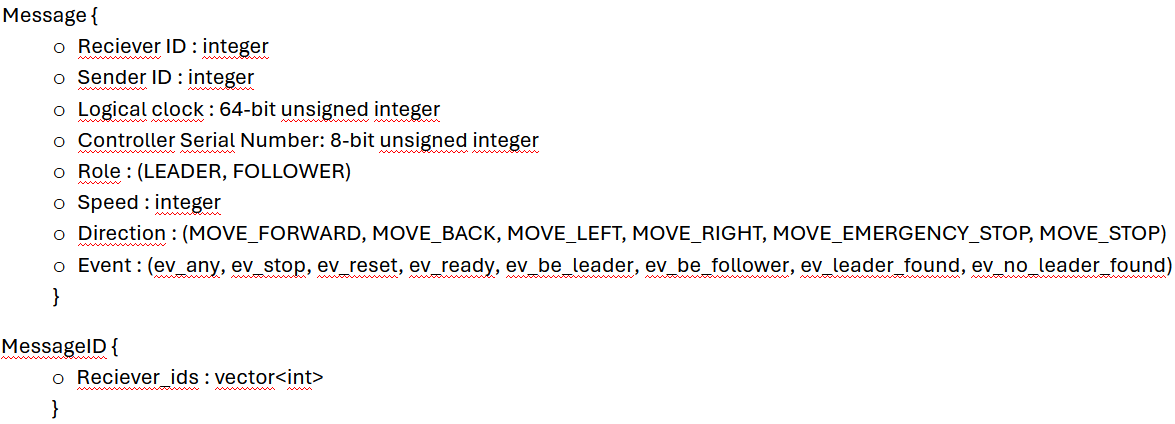
\includegraphics[width=0.4\textwidth]{images/message_messageid_structure.png}
    \caption{Message and MessageID structure}
    \label{img:message_messageid_structure}
\end{figure}

Each message contains the following fields (its structure is shown in Figure \ref{img:message_messageid_structure}):

\begin{itemize}
    \item Recipient ID: An integer uniquely identifying the intended receiver of the message within the fleet.
    \item Sender ID: An integer representing the ID of the truck from which the message originated.
    \item Logical clock: A 64-bit unsigned integer that ensures messages are processed in the correct chronological order, crucial in distributed systems where timing is key.
    \item Controller Serial Number: An 8-bit unsigned integer uniquely identifying a controller within a truck, used to direct messages appropriately in systems with multiple controllers.
    \item Role: An enumeration representing the truck's role within the fleet, with possible values of \texttt{LEADER} or \texttt{FOLLOWER}.
    \item \textbf{Speed:} An integer value indicating the truck's speed, for use in movement commands and status updates.
    \item Direction: An enumerated type indicating the truck's movement direction, with options such as \texttt{MOVE\_FORWARD}, \texttt{MOVE\_BACK}, \texttt{MOVE\_LEFT}, \texttt{MOVE\_RIGHT}, \texttt{MOVE\_EMERGENCY\_STOP}, and \texttt{MOVE\_STOP}.
    \item Event: An enumeration indicating the type of event associated with the message. Possible values include \texttt{ev\_any}, \texttt{ev\_stop}, \texttt{ev\_reset}, \texttt{ev\_ready}, \texttt{ev\_be\_leader}, \texttt{ev\_be\_follower}, \texttt{ev\_leader\_found}, and \texttt{ev\_no\_leader\_found}. These events trigger specific behaviors and state changes within the truck's control logic.
\end{itemize}

\subsection{MessageID Structure}
The \texttt{MessageID} structure is utilized when a message is intended for multiple recipients, enabling efficient broadcast communication:

\begin{itemize}
    \item Recipient IDs: A vector of integer IDs that specifies all the intended recipients of the message. This approach optimizes the communication process by reducing the number of messages sent over the network.
\end{itemize}

%% message Serialization and Deserialization 

\subsection{Serialization and Deserialization}

The utilization of the winsock2.h library within our communication system necessitates a reliable method for message exchange between different entities in the network. Due to the library's operating principle, which relies on the transmission of data streams over TCP/IP, it is imperative that complex data structures, such as those used in our system, are serialized into a stream of characters. JSON serialization offers a standardized and language-agnostic format for converting our message objects into a text-based format that can be easily transmitted over the network. Upon receipt, these character streams are then deserialized back into their original structured form, allowing for the seamless reconstruction and processing of the transmitted data.

\begin{figure}[ht]
    \centering
    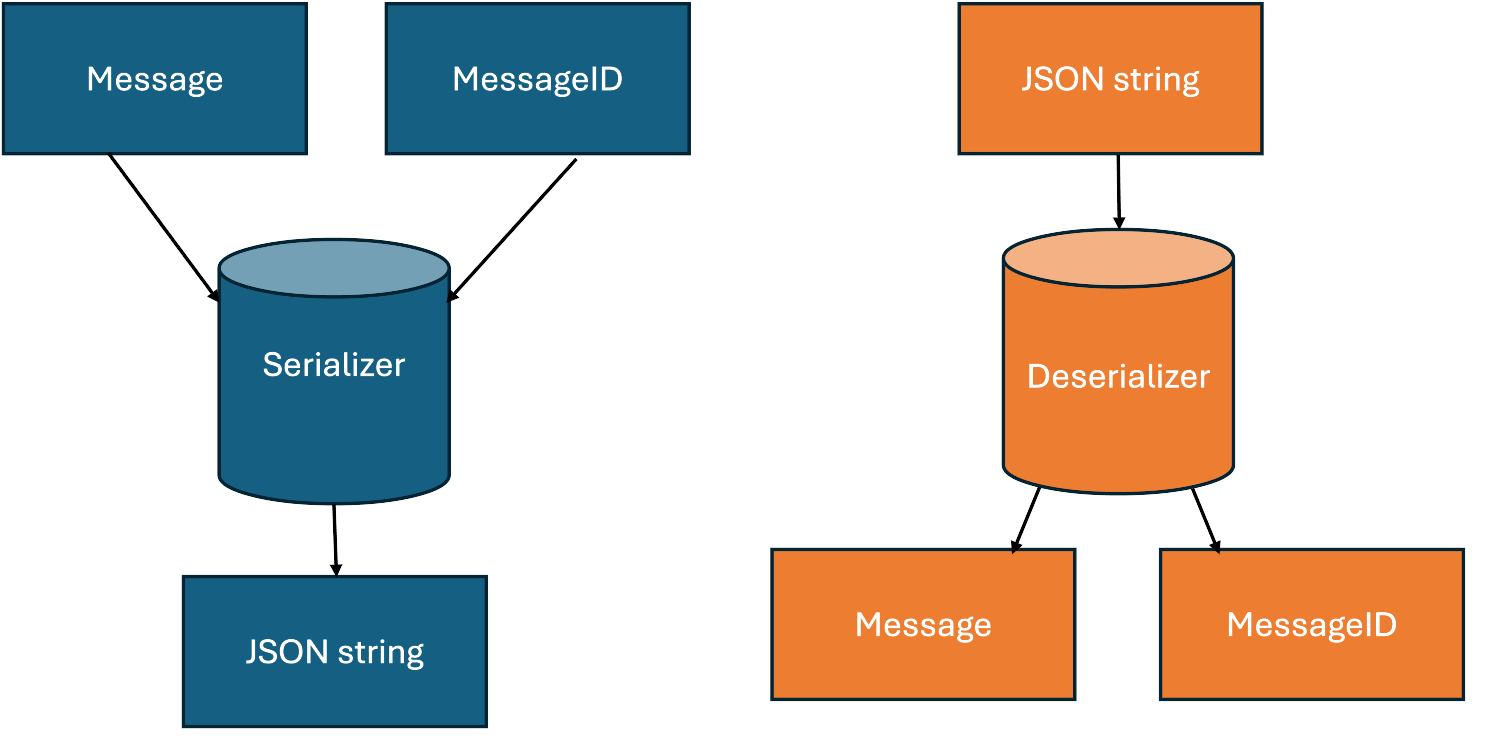
\includegraphics[width=0.4\textwidth]{images/serialization_deserialization.png}
    \caption{Serialization and Deserialization}
    \label{img:serialization_deserialization}
\end{figure}

\subsubsection{Serialization}
Serialization is the process of converting an object's state and data into a format that can be transmitted and then reconstructed later. In the context of our project, the \texttt{MessageParser} class is responsible for serialization and deserialization of \texttt{Message} and \texttt{MessageID} objects to and from JSON format.

The Serializer (see Figure~\ref{img:serialization_deserialization}) comprises \texttt{toJSON} and \texttt{toJSONID} methods which are responsible for serialization. They take \texttt{Message} and \texttt{MessageID} objects, respectively, and convert them into JSON strings.

\subsubsection{Deserialization}
Deserialization is the reverse process, where JSON strings are converted back into \texttt{Message} or \texttt{MessageID} objects.

The Deserializer consists of three important methods:

\begin{itemize}
    \item \texttt{fromJSONVariant} is an overloaded function that can return either a \texttt{Message} or \texttt{MessageID} object from a JSON string. It determines the type of object to deserialize based on the presence of specific keys in the JSON string.

    \item \texttt{fromJSON} parses a JSON string, extracting data to populate the fields of a \texttt{Message} object. It uses a \texttt{stringstream} to separate the JSON string into key-value pairs and then assigns these values to the appropriate fields of the \texttt{Message} object.
    
    \item \texttt{fromJSONMessageID} takes a JSON string that represents message IDs and extracts an array of receiver IDs, which it uses to populate a \texttt{MessageID} object.
    
\end{itemize}

\subsubsection{Utility Methods}
The class also includes utility methods for converting enumeration values to and from strings, which are used during serialization and deserialization:

\begin{itemize}
    \item \texttt{truckRoleToString} and \texttt{stringToTruckRole} convert between \texttt{truckRole\_e} enum values and their string representations.
    
    \item \texttt{directionToString} and \texttt{stringToDirection} handle the conversion for \texttt{MovementDirection} enums.
    
    \item \texttt{eventToString} and \texttt{stringToEvent} convert event types to and from strings.
\end{itemize}

The \texttt{MessageParser} class is a critical component that ensures the seamless transfer of complex objects between different parts of the system.
